\section{Qualitätsmessung der dekomprimierten Daten}
Bei verlustbehafteten Kompressionen muss die Qualität des dekomprimierten Bildes sichergestellt werden. Im optimalen Fall ähneln die dekomprimierten Daten ihren Originalen, sodass für das menschliche Auge keine Artefakte sichtbar sind.\\
Im Verlauf der Arbeit wurden zwei Metriken verwendet: Die Standardabweichung und eine angepasste PSNR-HVS-M. Für die ersten Tests wurde nur die Standardabweichung gemessen. Es stellte sich heraus, dass die Standardabweichung nicht ausreicht: Oszillationen um die Originallinie fallen nicht ins Gewicht. Der absolute Fehler bleibt klein, für das menschliche Auge jedoch sind solche Artefakte störend. Ein Beispiel für die Artefakte ist in Abbildung \ref{resultate:loesung1:dct:randbehandlung:jvhartefakte} im Abschnitt \ref{resultate:loesung1:ringing} zu finden. Wie die Standardabweichung berechnet wird, ist im Abschnitt \ref{testsetup:ablauf} beschrieben. Für weitere Tests wurde zusätzlich die PSNR-HVS-M Metrik berechnet. Die Metrik stammt aus der Bildverarbeitung. Das Ziel des Fehlermasses ist es, eine hohe Korrelation zwischen der Metrik und dem menschlichen Augenmass zu erreichen. Wie die PSNR-HVS-M Metrik angepasst und umgesetzt wurde, ist im Abschnitt \ref{testsetup:psnr} beschrieben.\\
Für die Messungen wurden spezielle Aufnahmen der Feldlinien gewählt. Wie die Aufnahmen ausgewählt wurden, ist im Abschnitt \ref{testsetup:auswahl_erhebung} beschrieben.

\subsection{Auswahl und Erhebung der Testdaten}\label{testsetup:auswahl_erhebung}
Die Testdaten sollen zu einem alle Randfälle abdecken, als auch durchschnittliche Fälle enthalten. Aus diesem Grund wurden insgesamt zehn Datensätze ausgewählt: Vier Datensätze mit hoher Sonnenaktivität, zwei mit wenig und vier zufällig. Für die vier Datensätzen mit hoher Aktivität wurde in den Jahren 2014 und 2013 nach den grössten Solare Flares gesucht. Für die Datensätze mit wenig Aktivität wurde das Gegenteil gemacht, nach Zeiträumen mit möglichst kleinen Solar Flares gesucht.\\
Die Feldlinien werden aber nur alle sechs Stunden berechnet und Solar Flares sind sehr spontane Ereignisse. Auch eine grosse Flare kann während den sechs Stunden angefangen und wieder aufgehört haben. Für die grossen Solar Flares wurde deshalb beachtet, dass die Datensätze vor dem Ereignis verwendet wurden. Grosse Solar Flares entladen das Feld, vor dem Ereignis ist das Magnetfeld komplexer.\\
[\baselineskip]
Wie im Abschnitt \ref{konzept:ist-komprimierung} beschrieben, wird bereits eine einfache verlustbehaftete Kompression durchgeführt. Für die Testdaten wurde diese entfernt, was die rohe Datenmenge entsprechend anwachsen liess auf etwa 10 MiBytes pro Aufnahme.

\subsection{Berechnung der Standardabweichung}\label{testsetup:ablauf}
Die dekomprimierte Linie ähnelt dem Original, wenn die Abweichung konstant und klein bleiben. Eine seltene, dafür grosse Abweichung kann das Aussehen massgebend verändern. Für diesen Fall wurde Die Standardabweichung ausgewählt. Das Mass bewertet seltene, grosse Abstände stärker.\\
Die originale und dekomprimierte Feldlinie können unterschiedliche Abtastraten aufweisen. Die Standardabweichung muss deshalb unabhängig von der Abtastrate berechnet werden.

\subsubsection{Allgemeiner Fall}
\begin{figure}[!htbp]
	\center
	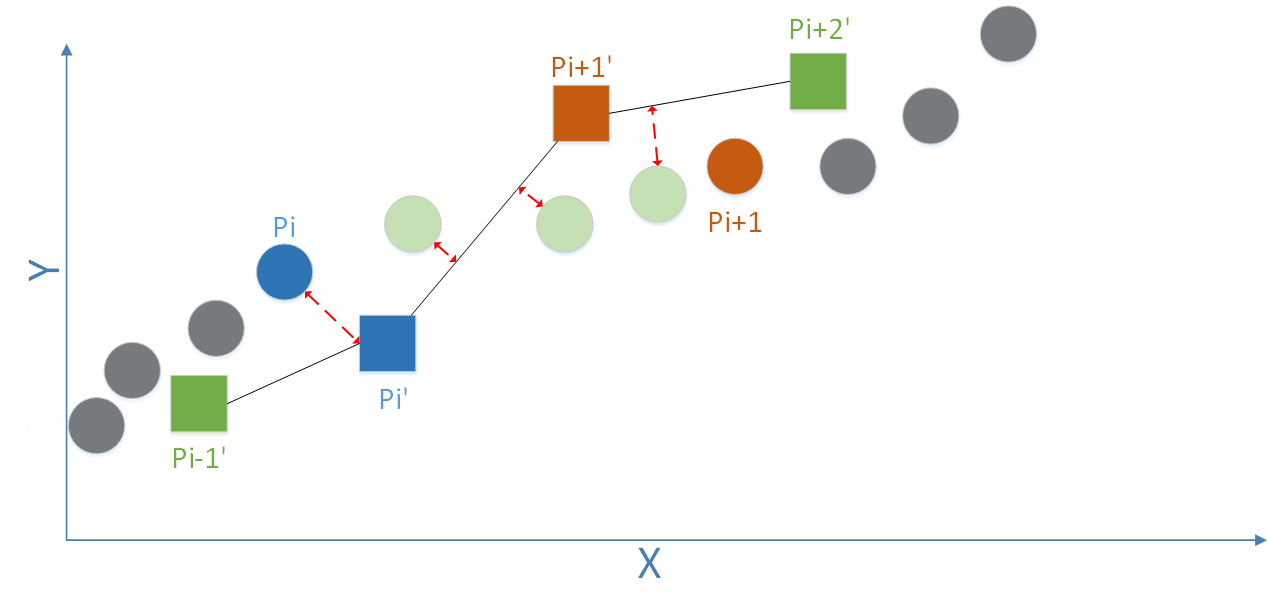
\includegraphics[width=0.8\textwidth,height=6cm,keepaspectratio]{./pictures/testsetup/errorcalc.png}
	\caption{Darstellung der Fehlerberechnung. Die Punkte sind die Originaldaten, die Quadrate sind die Punkte nach der Kompression.}
	\label{testsetup:ablauf:fehlerberechnung:diagramm}
\end{figure} 
Um die Abweichung unabhängig von der Abtastrate zu berechnen, wird zwischen den dekomprimierten Punkte eine Linie gezogen und den Abstand von dieser berechnet. Der Vorgang ist dargestellt im Diagramm der Abbildung \ref{testsetup:ablauf:fehlerberechnung:diagramm}. Für jeden Punkt $P1'$ aus den dekomprimierten Punkten $D$, nehme $P1'$ und den folgenden Punkt $P2'$. Ziehe eine Strecke $s$ durch $P1'$ und $P2'$. Suche von $p1'$ den Originalpunkt $P1$ aus allen Originalpunkten $O$ und rechne den Abstand aus zur Strecke $s$. Führe das für alle folgenden Originalpunkte durch, bis $P2$ erreicht wurde. Der Abstand $s$ zu $P2$ wird nicht mehr berechnet.\\
[\baselineskip]
Die Abstandsberechnung von Strecke $s$ zu einem Punkt $P$ erfolgt in zwei Schritten: Zuerst wird mit der Formel \eqref{testsetup:ablauf:formula:on_line} überprüft  , ob eine Senkrechte durch $P$ auf der Strecke $s$ zu liegen kommt. Falls das der Fall ist, wird der Abstand von $P$ zu $s$ berechnet \eqref{testsetup:ablauf:formula:distance}. Falls nicht, wird die kürzeste Distanz der Eckpunkte der Strecke zu $P$ berechnet.\\
\begin{equation} \label{testsetup:ablauf:formula:on_line}
 t = \frac{\vec{AB}*\vec{AP}}{\lvert \vec{AB}\rvert ^2} \quad 0 \leq t \leq 1
\end{equation}
\begin{equation}\label{testsetup:ablauf:formula:distance}
distance = \frac{\lvert \vec{BA}\times \vec{BP}\rvert}{\lvert \vec{BP} \rvert}
\end{equation}
$A$ und $B$ sind die Eckpunkte der Strecke. Falls $0 \leq t \leq 1$, existiert eine Senkrechte durch $P$ mit Fusspunkt auf der Strecke $s$. Die Distanz von $P$ zu $s$ wird mit der Formel \eqref{testsetup:ablauf:formula:distance} berechnet.\\
Wenn das nicht möglich ist, wird der kürzere Distanz von $P$ zu einem der Eckpunkte genommen. 

\subsubsection{Randbehandlung}
\begin{figure}[!htbp]
	\center
	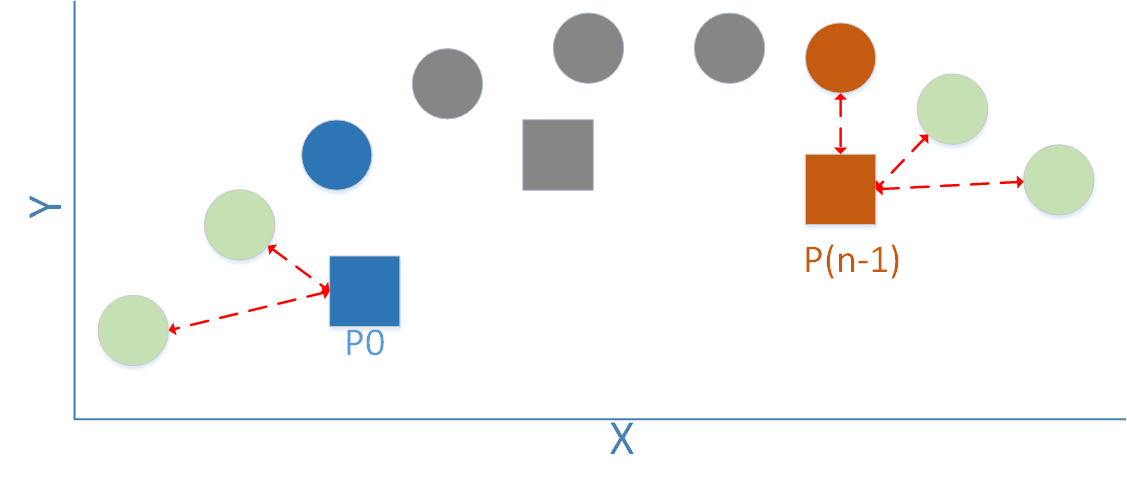
\includegraphics[width=0.8\textwidth,height=6cm,keepaspectratio]{./pictures/testsetup/randbehandlung.png}
	\caption{Darstellung der Fehlerberechnung. Die Punkte sind die Originaldaten, die Quadrate sind die Punkte nach der Kompression.}
	\label{testsetup:ablauf:randbehandlung:diagramm}
\end{figure}
Es ist möglich, dass die originalen Endpunkte der Feldlinien durch ein Subsampling verworfen wurden. Es ist möblich, dass am Anfang und am Ende Originalpunkte existieren, für die nie eine Distanz berechnet wurde. Das Diagramm der Abbildung \ref{testsetup:ablauf:randbehandlung:diagramm} zeigt das Problem. Deshalb müssen die Abstände der Eckpunkte von der Komprimierten- zur Original-Linie berechnet werden.

\subsubsection{Berechnung der Standardabweichung}
\begin{equation} \label{testsetup:ablauf:formula:deviation}
	\begin{split}
		\sigma(X)& = \sqrt(variance(X))\\
		variance(X) & = \sum{(x_i - E(x_i))^2}
	\end{split}
\end{equation}
Die Standardabweichung $\sigma$ einer Beobachtungsreihe $X$ $(x_1,x_2,x_3,\ldots, x_n-1)$ ergibt sich aus der Wurzel der Varianz von $X$. Die Varianz von $X$ kann errechnet werden, wenn man den Distanz jeder Beobachtung $x_i$ mit dem Erwartungswert $E(x_i)$ berechnet und quadriert. Die Beobachtung ist im diesen Fall ein Punkt der dekomprimierten Linie, während der Erwartungswert der Originalpunkt ist. Die Distanz wird mit dem besprochnen Verfahren \ref{testsetup:ablauf} berechnet. Die Summe der quadratischen Abstände ergibt die Varianz. Die Varianz wird über alle Testdaten berechnet, somit erhält man für einen Test einen Wert für die Standardabweichung.

\subsection{Berechnung der angepassten PSNR-HVS-M}\label{testsetup:psnr}
Die Peak-Signal-Noise-Ratio (PSNR) Metrik ist ein weitverbreitetes Fehlermass in der Bildverarbeitung. Es kann für die Messung des Fehlers zwischen dekomprimierten Bild und dem Original eingesetzt werden. Das Problem der Metrik ist aber, dass es nicht immer mit der menschlichen Wahrnemung korreliert. Ponomarenko et al.  \cite{ponomarenko2007between:psnr} haben eine modifizierte PSNR entwickelt; die PSNR Human Visual System Masking (HVS-M). In ihren Messungen erreichten sie eine hohe korrelation zwischen menschlicher Wahrnehmung von  verrauschten Bildern und dem neuen Fehlermass.\\
[\baselineskip]
\begin{equation} \label{testsetup:psnr:formula:psnr}
\begin{split}
PSNR & = 20 * log_{10}(MAX_I) - 10*log_{10}(MSE) \\
MSE & = \frac{1}{n}\sum_{i=0}^{N-1}[E(i)-D(i)]^2
\end{split}
\end{equation}
Die PSNR \eqref{testsetup:psnr:formula:psnr} setzt sich zusammen aus dem maximal möglichen Wert $MAX_I$ und dem ''Mean Squared Error´´ ($MSE$), der durchschnittliche Quadratische Fehler zwischen den Originaldaten $E()$ den dekomprimierten Daten $D()$.
Der Unterschied zwischen der PSNR und der PSNR-HVS-M liegt in der Berechnung des durchschnittlichen quadratischen Fehlers. Das Diagramm der Abbidlung \ref{testsetup:ablauf:psnr:flowchart} zeigt den Ablauf der neuen Berechnung.\\
\begin{figure}[!htbp]
	\center
	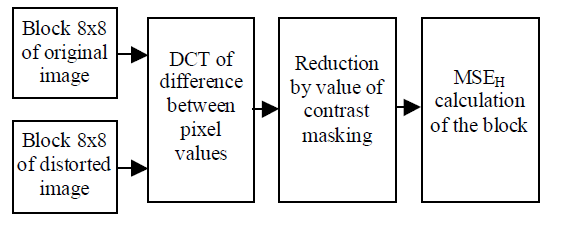
\includegraphics[width=0.8\textwidth,height=3.5cm,keepaspectratio]{./pictures/testsetup/psnr-hvs-m-flow.png}
	\caption{Flussdiagramm der PSNR-HVS-M Berechnung \cite{ponomarenko2007between:psnr}.}
	\label{testsetup:ablauf:psnr:flowchart}
\end{figure}
PSNR-HVS-M berechnet die Differenz zwischen dem Originalbild $E$ und dem verrauschtem Bild $D$ und führt die Daten mittels einer DCT in den Frequenzraum. Der nächste Schritt Contrast Maskin reduziert die Differenz, wenn das menschliche Auge den Frequenzunterschied nicht erkennen kann. Die Berechnung des $MSE_H$ Wertes erfolgt wieder gleich wie bei der PSNR.

\subsubsection{Contrast Masking}
Um das Contrast Masking zu berechnen, führt Ponomarenko et al. die gewichtete Energie der DCT Koeffizienten $E_w$ \eqref{testsetup:psnr:formula:weighted_energy}und den masking effect $E_m$ \eqref{testsetup:psnr:formula:masking_effect} ein:\\
\begin{equation}\label{testsetup:psnr:formula:weighted_energy}
 E_w(X)  = \sum_{i=0}^{7}\sum_{j=0}^{7}[X_{ij}]^2 C_{ij}
\end{equation}
\begin{equation} \label{testsetup:psnr:formula:masking_effect}
	E_m(X)  = \frac{1}{f_m}E_w(X)
\end{equation}
Wobei $X$ die Kosinus-Koeffizienten eines Bildblocks sind und $C$ die jeweiligen Gewichtungen zur Frequenz. Der Normalisierungsfaktor $f_m$ wurde experimentell ermittelt und auf $16$ festgelegt. Ponomarenko et al. argumentiert, dass der Unterschied zwischen einem Block $X_e$ und einem verrauschten Block $X_d$ unsichtbar sind, wenn die Formel \eqref{testsetup:psnr:formula:masking} erfüllt ist.
\begin{equation} \label{testsetup:psnr:formula:masking}
	E_w(X_e-X_d) < max[E_m(X_e),E_m(X_d)]
\end{equation}
Das Contrast Masking fliesst mit folgender Formel in die Distanzberechnung mit ein \eqref{testsetup:psnr:formula:error}.
\begin{equation} \label{testsetup:psnr:formula:error}
	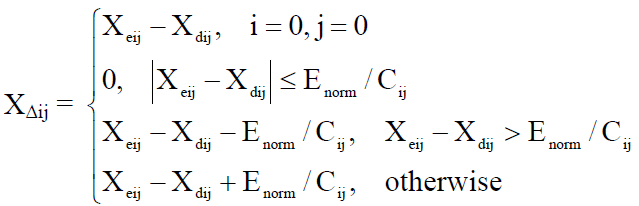
\includegraphics[scale=0.5]{./pictures/testsetup/mseH}\\
\end{equation}
Wobei $E_{norm} = \sqrt{max[E_m(X_e),E_m(X_d)] / 64}$. $X_{eij}$ ist der DCT Koeffizient des Originalblockes und $X_{dij}$ der Koeffizient des verrauschten Blockes. Dabei ist es irrelevant ob die DCT Koeffizienten subtrahiert werden oder wie in der Abbildung \ref{testsetup:ablauf:psnr:flowchart} angedeutet, zuerst die Differenz der Pixelwerte berechnet und diese DC transformiert. Beide Wege führen zum selben Resultat. Aus den Distanzen $X_{\Delta ij}$ wird die PSNR \eqref{testsetup:psnr:formula:psnr} berechnet.\\
[\baselineskip]
Wie gut die PSNR-HVS-M Metrik mit dem menschlichen Auge übereinstimmt, hängt vom Normalisierungsfaktor $f_m$ und von der Wahl der Gewichtungen $C$ ab. Ponomarenko et al. verwendeten die normalisierten ($\frac{10}{x}$) und quadrierten Werte der Standard JPEG Quantisierungsmatrix \cite{wallace1992jpeg}. Es ist zu beachten, dass der DC-Koeffizient nicht im Contrast Masking berücksichtigt wird, für den Wert wird die normale PSNR berechnet. Der DC-Koeffizient stellt die durchschnittliche Helligkeit in einem Block dar. Das menschliche Auge kann auch kleine Unterschiede in dieser Frequenz erkennen.

\subsubsection{Umsetzung und Anpassung der PSNR-HVS-M für diese Arbeit}
Der grösste Unterschied zur Arbeit von Ponomarenko et. al. ist der Einbezug des DC-Koeffizienten ins Contrast-Masking. Das menschliche Auge kann leichte Verschiebungen der Feldlinien kaum unterscheiden. Des weiteren musste für die Feldlinie eine eigene Quantisierungsmatrix gefunden werden, ausdenen die Gewichtungen berechnet werden. Die Quantisierungsmatrix wurde empirisch ermittelt, sodass die dekomprimierten Feldlinien keine sichtbaren Artefakte aufweisen.\\
Für die PSNR wird der maximale Wert $MAX_I$ benötigt. Hier wurde der maximal mögliche Wert der PFSS Simulation verwendet, den vierfachen Sonnenradius.\\
Der letzte Wert, den es zu setzen gibt, ist der Normalisierungsfaktor $f_m$. Ponomarenko et. al. schrieb keine zusätzliche Information oder Begründung zu diesem Wert. Dieser Wert stellt ein, wie stark das Contrast-Masking einfliessen soll. Je höher der Wert ist, desto ähnlicher ist die PSNR-HVS-M Metrik der normalen PSNR.\\
Die Tabelle \ref{testsetup:psnr:umsetzung:tabelle:f_m} erforscht den Einfluss des $f_m$ Faktors. Dazu wurde die PSNR-HVS-M zu drei dekomprimierten Simulationen berechnet, welche eine unterschiedliche Qualität aufweisen. 
\begin{table}
\center
\begin{tabular}{r|c|c|c}
	Qualität &$f_m$ 8 &$f_m$ 16 &$f_m$ 32 \\\hline
	Keine sichtbare Artefakte & 96.8 dB & \textbf{95.6} dB& 94.5 dB \\
	Kaum sichtbare Artefakte & 95.8 dB & \textbf{94.4} dB& 93.3 dB\\
  Sichtbare Artefakte & 90.0 dB & \textbf{88.3} dB & 87,0 dB
\end{tabular}
\caption{Einfluss des $f_m$ Faktors auf die PSNR-HVS-M.}
\label{testsetup:psnr:umsetzung:tabelle:f_m}
\end{table}
Für diesen Anwendungsfall scheint der Faktor $f_m$ sich stabil zu verhalten: der Faktor kann verdoppelt oder halbiert werden und die resultierenden Distanzen bleiben in der selben Grössenordnung. Es wurde der Standardwert von $16$ übernommen. Eine Anpassung von $f_m$ scheint nicht die Metrik massgebend zu verändern und hat vermutlich weniger Einfluss als die Gewichtung der DCT Koeffizienten. \\
[\baselineskip]
Die PSNR-HVS-M ist nicht unabhängig von der Abtastrate. Es erwartet, dass die zu vergleichenden Datenmengen gleich viele Punkte enthalten. Für diese Arbeit werden die Originaldaten auf die selbe Punktmenge reduziert. Wenn pro Feldlinie exakt ein Punkt abgespeichert wird, würde die PSNR-HVS-M trotzdem eine hohe Ähnlichkeit zwischen Original und dekomprimierten Feldlinien ergeben. Dies ist Vertretbar, da die Standardabweichung eine hohe Distanz ergeben würde. Die PSNR-HVS-M soll hauptsächlich Artefakte aufdecken, welche in der Standardabweichung nicht ins Gewicht fallen wie die Ringing Artefakte vom Abschnitt \ref{resultate:loesung1:ringing}.